% ===========================================================================
% Section 3: the floorline -- a roofline-inspired lower bound on the
% unavoidable overhead of a parallelism strategy, used to choose between
% gsplit, DGL (data parallel), and the pipeline.
% Assumptions are typeset in red via \assume{...}; author-softenable
% weaknesses via \flag{...}.
% ===========================================================================
\providecommand{\assume}[1]{{\color{red}#1}}
\providecommand{\flag}[1]{{\color{red}#1}}

\section{A Lower Bound on Overhead}
\label{sec:roofline}
\label{sec:simulator}   % keeps existing \ref{sec:simulator} links alive
\label{sec:floorline}

\paraq{What is this section for?}
In Sections~\ref{sec:limitations} and~\ref{sec:hybrids} we saw that the best choice between
data-parallel (DGL), split (gsplit), and pipeline training depends on the model (depth, hidden
size), the graph, and the hardware (compute throughput, interconnect bandwidth). This section
explains that choice with a simple construction: we plot each strategy's \emph{overhead} as a
lower-bound curve and read off which strategy pays less. The picture borrows the two-resource,
ridge-and-crossover shape of the roofline~\cite{williams2009roofline}, but because it bounds
overhead from below rather than throughput from above, we call it a \emph{floorline}. The side of
its ridge on which a layer falls names the strategy with the smaller overhead.

\paraq{Why overhead, and not throughput?}
The useful work of a mini-batch -- each distinct output row computed once -- is the same whichever
strategy runs it. What differs is the \emph{overhead} each strategy adds on top: DGL recomputes
rows on several GPUs, gsplit moves rows across the interconnect, the pipeline hides the move behind
compute. Plotting useful throughput would spend the picture on a quantity that does not change
between strategies and hide the decision inside correction factors. We therefore model the one
thing that does change -- the overhead -- and compare the two overheads directly. The whole
construction is built from a single sampling pass (minutes of CPU per setting) plus one set of
microbenchmarks per GPU. The model is deliberately simple: its assumptions are listed once, up
front, and we refine them only where a measurement asks for it.

% ---------------------------------------------------------------------------
\subsection{Assumptions}
\label{sec:cm-assumptions}

\paraq{Which assumptions does the model make?}
\begin{enumerate}\itemsep1pt
  \item[\assume{(A1)}] \assume{\textbf{Two costs per layer.} A layer costs useful dense work plus,
        depending on the strategy, one overhead: redundant work (DGL) or a shuffle (gsplit). Within
        a layer the neighbour gather and the dense arithmetic overlap, so the slower sets the
        compute time. Compute and shuffle overlap only in the pipeline; gsplit serialises them.}
  \item[\assume{(A2)}] \assume{\textbf{Steady state, fixed rates.} Latency, kernel launches, and
        synchronisation are ignored; one measured rate per resource and hidden size, the same for
        every layer.}
  \item[\assume{(A3)}] \assume{\textbf{Training step.} Modelled time is forward plus backward:
        compute counts $3\times$ the forward FLOPs ($2\times$ for the input layer) and the shuffle
        $2\times$ the forward bytes (rows out, gradients back).}
  \item[\assume{(A4)}] \assume{\textbf{Busiest GPU.} Per mini-batch the per-GPU maxima of rows,
        edges, and shuffled rows stand for the slowest GPU; strategies are compared per useful row.}
  \item[\assume{(A5)}] \assume{\textbf{Pipeline.} Its two micro-batches are identical and overlap
        perfectly.}
\end{enumerate}

% ---------------------------------------------------------------------------
\subsection{One floorline: redundant compute versus the shuffle}
\label{sec:cm-floor}

\paraq{What is the overhead of each strategy?}
Let $F$ be the useful dense FLOPs of a layer on the busiest GPU and $S$ the bytes that GPU would
shuffle under gsplit. Both strategies pay the useful $F$; we subtract it and keep only the
overhead. gsplit adds the shuffle. DGL adds the redundant dense work: it recomputes rows that other
GPUs also compute, a factor $\rho \ge 0$ of extra FLOPs, so
\begin{equation}
  F_{\mathrm{dgl}} = (1+\rho)\,F ,\qquad
  t^{\mathrm{over}}_{\mathrm{dgl}} = \frac{\rho F}{\hat P},\qquad
  t^{\mathrm{over}}_{\mathrm{gs}} = \frac{S}{\hat B},
  \label{eq:floor-overheads}
\end{equation}
with $\hat P$ the dense rate and $\hat B$ the interconnect bandwidth. We keep $\rho$ abstract; how
it is measured is deferred to Section~\ref{sec:cm-estimate}. The point of writing the overheads
this way is that the choice is now a comparison of two numbers.

\paraq{What is the floorline?}
The least overhead the layer can pay, having chosen the better strategy, is
\begin{equation}
  t_\star = \min\!\big(t^{\mathrm{over}}_{\mathrm{dgl}},\ t^{\mathrm{over}}_{\mathrm{gs}}\big)
          = \min\!\Big(\frac{\rho F}{\hat P},\ \frac{S}{\hat B}\Big).
  \label{eq:floor-min}
\end{equation}
Put the \emph{redundant-work intensity} $x = \rho F / S$ on the $x$-axis -- redundant FLOPs per
shuffled byte -- and the overhead per shuffled byte, $y = t_\star/S$, on the $y$-axis:
\begin{equation}
  y(x) = \min\!\Big(\frac{x}{\hat P},\ \frac{1}{\hat B}\Big).
  \label{eq:floorline}
\end{equation}
This is the floorline: a rising branch $x/\hat P$ (DGL's overhead, growing with redundancy) that
plateaus into a flat branch $1/\hat B$ (gsplit's shuffle, independent of redundancy). The two meet
at the \textbf{ridge}
\begin{equation}
  x^\star = \frac{\hat P}{\hat B}.
  \label{eq:ridge}
\end{equation}

\begin{figure}[h]
\centering
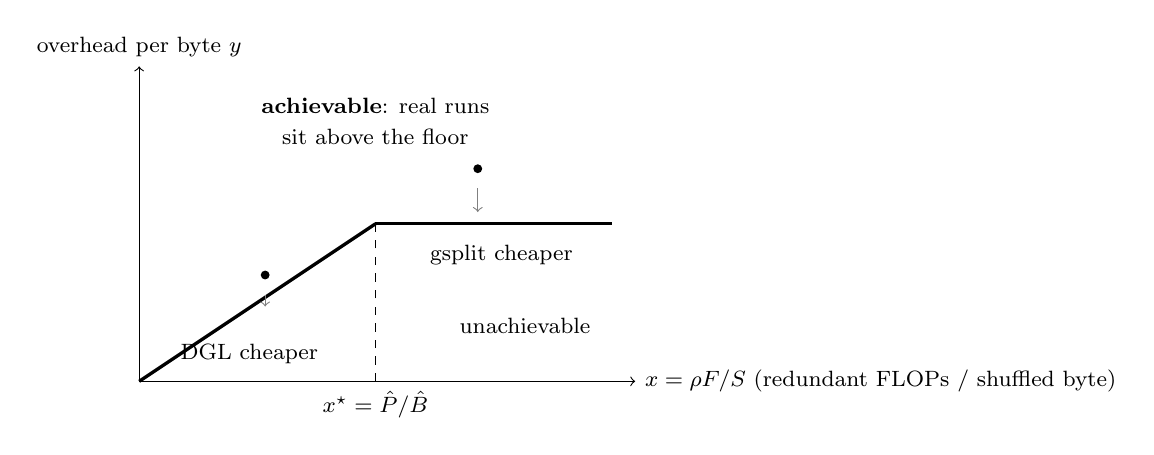
\begin{tikzpicture}[scale=1.0]
  % axes
  \draw[->] (0,0) -- (6.3,0) node[right] {\footnotesize $x=\rho F/S$ (redundant FLOPs / shuffled byte)};
  \draw[->] (0,0) -- (0,4.0) node[above] {\footnotesize overhead per byte $y$};
  % ridge x-coordinate
  \def\xr{3.0}
  \def\yr{2.0}
  % DGL rising branch up to ridge
  \draw[very thick] (0,0) -- (\xr,\yr);
  % gsplit flat branch after ridge
  \draw[very thick] (\xr,\yr) -- (6.0,\yr);
  % ridge marker
  \draw[dashed] (\xr,0) -- (\xr,\yr);
  \node[below] at (\xr,0) {\footnotesize $x^\star=\hat P/\hat B$};
  % region labels
  \node at (1.4,0.35) {\footnotesize DGL cheaper};
  \node at (4.6,1.6) {\footnotesize gsplit cheaper};
  % achievable region (above floor)
  \node[align=center] at (3.0,3.3) {\footnotesize \textbf{achievable}: real runs\\[-1pt] \footnotesize sit above the floor};
  \node at (4.9,0.7) {\footnotesize unachievable};
  % sample actual points above the floor
  \fill (1.6,1.35) circle (1.6pt);
  \fill (4.3,2.7) circle (1.6pt);
  \draw[->,gray] (1.6,1.1) -- (1.6,0.95);
  \draw[->,gray] (4.3,2.45) -- (4.3,2.15);
\end{tikzpicture}
\caption{The floorline (thick) is a lower bound on a layer's overhead per shuffled byte: the rising
branch is DGL's redundant compute, the flat branch is gsplit's shuffle, and they cross at the ridge
$x^\star=\hat P/\hat B$. Real runs pay more than the model's best-case rates, so measured points sit
\emph{above} the floor; nothing is achievable below it. Only the \emph{side of the ridge} is read:
left of it DGL pays less, right of it gsplit does.}
\label{fig:floorline}
\end{figure}

\paraq{What does the floor mean, and where does real performance sit?}
Equation~\eqref{eq:floorline} is built from best-case rates: peak $\hat P$, peak $\hat B$, no
latency, no launch cost (A2). It is therefore a genuine \emph{lower bound} -- no run can pay less
overhead than this. A real run pays more: sub-peak kernels, all-to-all latency and
synchronisation, feature loading. So on Figure~\ref{fig:floorline} every measured point lies
\emph{above} the floor; the region below it is unachievable. The gap between a point and the floor
is the model's optimism, and we do not try to predict it -- it is exactly the part we chose not to
model. What the floorline is used for is not the height of a point but the \textbf{side of the
ridge} it falls on:
\begin{equation}
  \boxed{\ \text{DGL beats gsplit at a layer}\iff \rho\,\frac{F}{S} < \frac{\hat P}{\hat B}
         \iff x < x^\star.\ }
  \label{eq:floor-rule}
\end{equation}
Left of the ridge the shuffle is the larger cost, so recomputing is cheaper and DGL wins; right of
it redundancy is the larger cost, so moving rows is cheaper and gsplit wins. The interconnect moves
the ridge; the model, depth, and hidden size move $x$ (redundancy grows with depth, $F/S$ with
hidden size). A hybrid with split point $k$ is DGL below $k$ and gsplit above it; it wins when the
rule changes sign across the layers of one model (Section~\ref{sec:cm-layers}).

% ---------------------------------------------------------------------------
\subsection{Which two resources? A second floorline}
\label{sec:cm-second}

\paraq{Why is there more than one floorline?}
The construction compares the shuffle against \emph{redundant work}, but redundant work can bind on
either of two resources: the dense units (redundant FLOPs, above) or HBM (redundant random gather
of neighbour rows). The interesting modelling choice is which pair of resources to pit against the
shuffle. Replacing redundant FLOPs with redundant gather bytes $S_{\mathrm{g}}$ against the HBM rate
$\hat B_{\mathrm{m}}$ gives a second floorline on the same axes,
\begin{equation}
  y_{\mathrm{m}}(x_{\mathrm{m}}) = \min\!\Big(\frac{x_{\mathrm{m}}}{\hat B_{\mathrm{m}}},\
        \frac{1}{\hat B}\Big),\qquad
  x_{\mathrm{m}} = \frac{\rho\,S_{\mathrm{g}}}{S},\qquad
  x^\star_{\mathrm{m}} = \frac{\hat B_{\mathrm{m}}}{\hat B}.
  \label{eq:floor-mem}
\end{equation}
Since the gather and the dense work of a layer overlap (A1), DGL's overhead is the larger of the
two redundant costs, so DGL wins only when it is below the shuffle on \emph{both} floorlines;
gsplit wins as soon as it is cheaper on \emph{either}. In almost every setting the dense branch
binds, so the compute floorline~\eqref{eq:floorline} decides; the one place the gather binds is the
outermost layer of 4-layer GAT on products, where the second floorline~\eqref{eq:floor-mem} takes
over. Naming both resources is what makes the single-floorline rule precise.

% ---------------------------------------------------------------------------
\subsection{Estimating the counts}
\label{sec:cm-estimate}

\paraq{How are $\rho$, $F$, and $S$ obtained?}
One sampling pass replays the loaders of DGL, gsplit (with and without a data-parallel prefix), and
the pipeline, without features or training. For each layer it records, on the busiest GPU (A4), the
destination rows $n$, source rows $n_{\mathrm{src}}$, edges $e$, and shuffled rows $m$, plus the
distinct destination rows pooled across the GPUs. The dense FLOPs $F$ and shuffle bytes $S$ follow from
these counts and the per-model constants (Table~\ref{tab:cm-constants}), scaled by the training-step
factors (A3). The redundancy $\rho$ is the ratio of rows a strategy pays for to rows the mini-batch
needs: DGL's per-GPU frontiers overlap, so it recomputes rows; gsplit's partitions are disjoint, so
its $\rho$ is only the load imbalance of the busiest GPU above the mean. gsplit and the hybrids use a
global mini-batch of $1024$ seeds split across $4$ GPUs by partition; DGL gives each GPU $256$. The
three rates $\hat P$, $\hat B_{\mathrm{m}}$, $\hat B$ come from microbenchmarks
(Table~\ref{tab:cm-microbench}).
For GAT the shuffle moves narrow rows of the transformed features $z$, whose small-message
all-to-all runs below the measured peak bandwidth; we scale GAT's modelled shuffle time by a single
calibration constant to absorb this, fixed once on the sweep (Section~\ref{sec:results}).

\begin{table}[h]
\centering
\caption{Model constants (forward pass), read off DGL's \texttt{SAGEConv}/\texttt{GATConv}:
$\kappa$ gathered rows per edge, $\beta$ matrix--vector and $\gamma$ vector--vector products per
edge/destination/source row.}
\label{tab:cm-constants}
\small
\begin{tabular}{l c c c c c c c}
\toprule
Model & $\kappa$ & $\beta_e$ & $\beta_n$ & $\beta_s$ & $\gamma_e$ & $\gamma_n$ & $\gamma_s$ \\
\midrule
SAGE & 1 & 0 & 2 & 0 & 0 & 0 & 0 \\
GAT  & 1 & 0 & 0 & 1 & 1 & 1 & 1 \\
\bottomrule
\end{tabular}
\end{table}

\begin{table}[h]
\centering
\caption{Measured rates on one A100-SXM4-80GB node (fp32, TF32 off; $10^5$ rows, fanout $15$;
all-to-all over $4$ GPUs). Raw data: \texttt{results/microbench/}.}
\label{tab:cm-microbench}
\footnotesize
\begin{tabular}{l l c c c c c}
\toprule
Rate & Microbenchmark & $h{=}256$ & $512$ & $1024$ & $2048$ & $4096$ \\
\midrule
$\hat P$ (TFLOP/s) & layer GEMM on a sampled block
  & 15.0 & 18.7 & 19.0 & 19.1 & 19.1 \\
$\hat B_{\mathrm{m}}$ (GB/s) & neighbour gather (CSR SpMM)
  & 1206 & 1240 & 1259 & 1263 & 1281 \\
$\hat B$ (GB/s), PCIe-emu & NCCL all-to-all
  & 12.2 & 13.1 & 13.3 & 13.3 & 13.3 \\
$\hat B$ (GB/s), NVLink & NCCL all-to-all
  & 154 & 177 & 185 & 196 & 200 \\
\bottomrule
\end{tabular}
\end{table}

% ---------------------------------------------------------------------------
\subsection{From one layer to the whole model}
\label{sec:cm-layers}

\paraq{How is a split point chosen across layers?}
Rule~\eqref{eq:floor-rule} is per layer. Redundancy $\rho$ grows with distance from the seeds, so
the layers nearest the seeds are the smallest and least redundant and the layers farthest away are
the largest. We therefore read the layers from the output back towards the seeds and stop at the
first that prefers DGL: every layer above it is smaller and also prefers DGL, so it inherits the
choice. The split point $k$ is where the rule flips.
\begin{quote}\small
\texttt{for}\ $\ell = L, L{-}1, \dots, 1$:\quad
\texttt{if}\ layer $\ell$ prefers DGL (Eq.~\ref{eq:floor-rule}) \texttt{then}\ split point $k=\ell$,
\texttt{stop}.
\end{quote}
A pure strategy is the boundary case: $k=0$ is gsplit, $k=L$ is DGL.

\paraq{Where does the pipeline fit?}
The pipeline is the same floorline with one change. Write the full compute and shuffle times of a
layer as
\begin{equation}
  T^{\mathrm{cmp}} = \frac{(1+\rho)\,F}{\hat P},\qquad
  T^{\mathrm{net}} = \frac{S}{\hat B},
  \label{eq:layer-times}
\end{equation}
the useful dense work $F/\hat P$ inflated by redundancy, and the shuffle. DGL pays
$T^{\mathrm{cmp}}$ (no shuffle) and gsplit pays $T^{\mathrm{cmp}}+T^{\mathrm{net}}$ serially; the
pipeline overlaps them (A5), so its layer costs $\max(T^{\mathrm{cmp}},T^{\mathrm{net}})$, with the
redundancy of its two micro-batches, $\rho_{\mathrm{pipe}}$, in place of $\rho$. Substituting
$\rho_{\mathrm{pipe}}$ and the overlap into
Equations~\eqref{eq:floor-overheads}--\eqref{eq:floor-rule} reproduces the whole construction, so we
do not redraw it. The choice is between the pipeline and gsplit, and because compute is typically
large enough to hide the shuffle, the pipeline's overhead collapses to its redundant compute alone;
the comparison then turns on $\rho_{\mathrm{pipe}}$, and we make the choice at the bottom (largest)
layer, as above.

\paraq{What does this section conclude?}
The floorline is a roofline-inspired lower bound on a strategy's overhead: a rising redundant-work
branch and a flat shuffle branch crossing at a ridge fixed by the interconnect. The useful work is
the same for every strategy, so only the overhead and the side of the ridge matter; real runs sit
above the floor and are not predicted. Built from one sampling pass and three measured rates, the
rule picks a strategy per layer, a split point across layers, and the pipeline-versus-gsplit choice
at the bottom layer. Section~\ref{sec:res-table} reports how often the pick matches the measured
winner.
